\documentclass[tikz,border=8pt]{standalone}

\usepackage{tikz}
\usetikzlibrary{arrows.meta, positioning, fit, backgrounds}

\tikzset{
  place/.style={circle, draw, thick, minimum size=12mm, align=center, font=\small},
  transition/.style={rectangle, draw, thick, minimum width=16mm, minimum height=7mm, align=center, font=\small, fill=black!4},
  note/.style={font=\small, align=left},
  phase/.style={rounded corners, draw, dashed, inner sep=6mm, fill=black!2},
  flow/.style={-Latex, thick},
}

\begin{document}
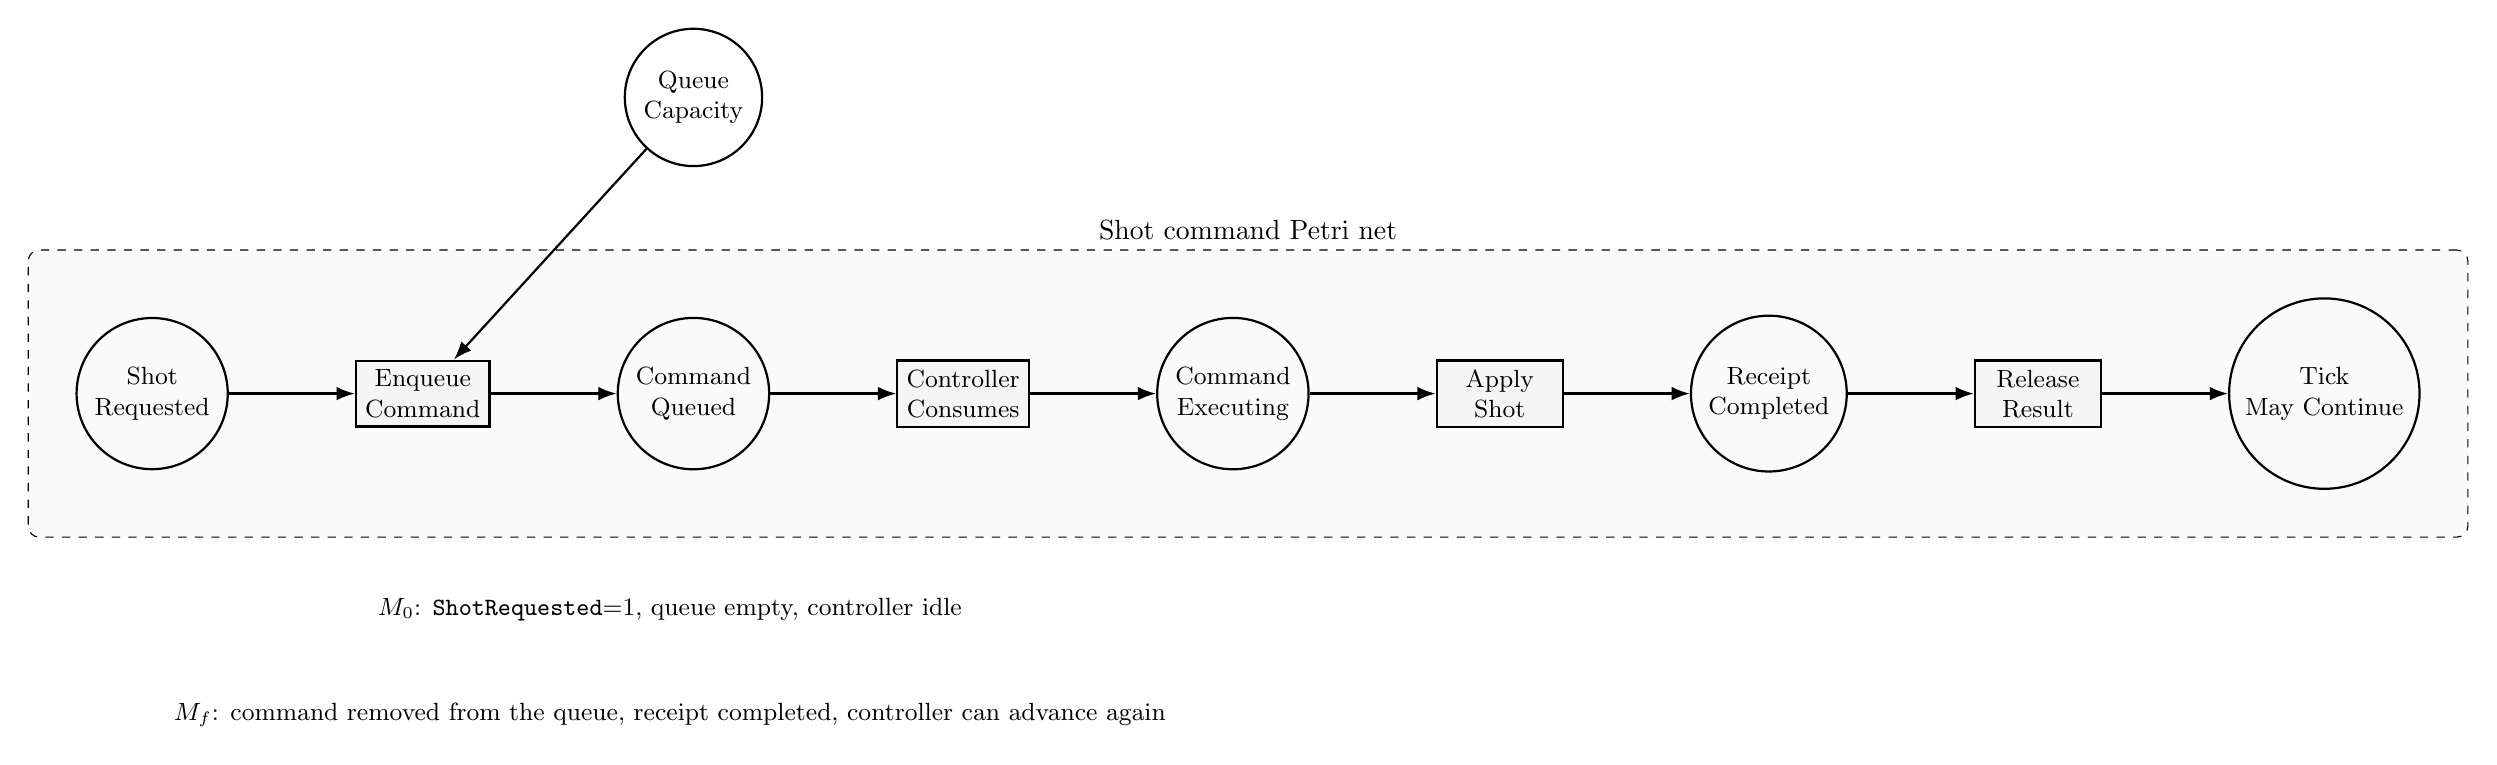
\begin{tikzpicture}[node distance=18mm and 16mm]
  \node[place] (request) {Shot\\Requested};
  \node[transition, right=of request] (queue) {Enqueue\\Command};
  \node[place, right=of queue] (queued) {Command\\Queued};
  \node[transition, right=of queued] (consume) {Controller\\Consumes};
  \node[place, right=of consume] (executing) {Command\\Executing};
  \node[transition, right=of executing] (apply) {Apply\\Shot};
  \node[place, right=of apply] (result) {Receipt\\Completed};
  \node[transition, right=of result] (release) {Release\\Result};
  \node[place, right=of release] (done) {Tick\\May Continue};

  \draw[flow] (request) -- (queue);
  \draw[flow] (queue) -- (queued);
  \draw[flow] (queued) -- (consume);
  \draw[flow] (consume) -- (executing);
  \draw[flow] (executing) -- (apply);
  \draw[flow] (apply) -- (result);
  \draw[flow] (result) -- (release);
  \draw[flow] (release) -- (done);

  \node[place, above=of queued, yshift=1mm] (capacity) {Queue\\Capacity};
  \draw[flow] (capacity) -- (queue);

  \node[note, below=15mm of queued, xshift=-3mm] (initial) {$M_0$: \texttt{ShotRequested}=1, queue empty, controller idle};
  \node[note, below=8mm of initial] (final) {$M_f$: command removed from the queue, receipt completed, controller can advance again};

  \begin{scope}[on background layer]
    \node[phase, fit=(request)(done), label=above:{Shot command Petri net}] {};
  \end{scope}
\end{tikzpicture}
\end{document}
